%===================================== CHAP 8 =================================

\chapter{Evaluation}

\section{Process}
\label{evaluationProcess}
This sections contains evaluation of the process. This includes both the methodology, development and challenges the group has met and resolved.

\subsection{Methodology}
\label{evaluationMethodology}
During the project the group utilized scrum (see \ref{methodology}) with sprints, daily stand-up meetings and retrospectives, this worked well and led to all group members being aware of what the others were working on. 

The two weeks sprints worked well, this was enough time to finish features in all but one sprint. This were in sprint two were the group had some problems (see \ref{sprint2}) concerning technology and under estimating of tasks. During the sprints the daily stand-up meetings helped the scrum master and other group members to be updated, and to prioritize the work remaining during each sprint. 

To visualize the progress of the project, and see who were working on what, as well as to keep track of the different milestones, the group used Waffle.io (see section \ref{Waffle.io}) which worked great. The customer also had full access to the Waffle panel, were he could easily follow the project's progress, and add new milestones and issues to the project.

From Extreme Programming the group used pair programming. This was very effective, because the pairs learned from each other as well as more than one member were aware of the status of the feature. 




\subsection{Development}

The development was influenced on the process, methodology and the customer. The group developed in an iterative manner, and tried to have new features to show the customer every week. Biweekly the group updated the live server with a new release. This way of developing worked very well. It made it possible for the group to focus on few set of features while they were working, and finalize them before they started working on new features. Some features was more time consuming than others and some of the features demanded that the group had to acquire new knowledge. 

To keep track of the features that was to be developed, the group used GitHub and Git to maintain the code. Every features was developed on separated branches, and then merged with the main developing branch when a feature was done. This was done up to several times during each sprint. When a sprint was finished the master branch was updated, which updated the production server. The customer appreciated that the application was rapidly updated on the production server, because he could test it whenever he wanted and give the group feedback throughout the entire project period. The group also found this very helpful, because it helped them to prioritize which features that should be implemented next, as well as fixing any bugs that occurred.


\subsection{Challenges}
The group has encountered a few challenges during the project.

As the group had decided to utilize new frameworks, libraries and working- and testing methodes, some issues did occure. The entire group had some previous experience with Python, Javasript, HTML5 and CSS, but not very much experience with Django, React and Redtux (see section \ref{frontEnd} and \ref{backEnd}). Since all of this was new, the group spent a lot of time learning how to use to tools in a good and efficient way. 

During sprint 2 the group had some huge problems getting started with Flux \cite{flux}. The group spent a lot time trying to set up a good working environment with Flux, but could not manage to do so. After some research, the decision felt on using Redux instead. There was some problems getting this working as well, but after a short period of time, the application was running smoothly with Redux. 

Another challenge was to work together as much as planned. There was challenges with planning the group timetable. When could all group members meet, so that the meeting would not collide with other subjects. As well as planning when everyone could meet, it was a challenge to work this many people at the same project over the project's period. This many people combined with new ways of working offered some small challenges throughout the entire project, but no anything that led to dissatisfaction within the group. 

With the customer and users, the group faced a problem concerning how to present the facilitation for users. The customer was worried about hurting someones feelings by using symbols and words that described for whom an activity was facilitated for. After the second workshop (see section \ref{focusGroup}), the users actually just wanted describing standard symbols, that said if the activity was suited for them or not.  

Another challenge with the customer was that he was constantly changing the requirements. At every meeting there was always something new that he had a new idea that got the highest priority for the upcoming week. Sometimes this was very stressful, but the group did a good job satisfying the customer.  

\section{Cooperation With Customer}
From the very beginning the group started cooperating closely with the customer. Every week through out the entire project the group met with the customer (see section \ref{ss:customer_meetings} and examples in appendix \ref{meeting_minutes_customer_meetings}). Throughout the entire project the customer was very engaged to the project. He arranged workshops (see section \ref{WorkshopUserAndProviders} and section \ref{focusGroup}) with users and was attending them as well. The customer also arranged a focus group with possible providers for the application (see section \ref{focusGrouoProviders}). This was very helpful for the group, because the users gave valuable feedback for the group and made it easier to create an application that actually would turn out to be something that users would like to use. 

\section{Group Collaboration}
Since the start of the project, the group have been very motivated to work hard with this project and has strived to satisfy the customer as much as possible. All of the group-members knows each other and have worked together in previous projects, therefore the group collaborated very well through out the project and there has not been any big problems with communication within the group. If any misunderstandings came up within the group eighter about the product, development or anything else, everyone discussed the issue and the group quickly came up with a solution. In regards of the development, the group collaborated very well together. If any issues came up, non of the members hesitated to ask for help from others. In several cases the members of the group also took the advantage of pair-programming to learn from each other and to achieve the best possible result.

\section{Project Management}
\subsection{Risk Analysis}
\label{updated_risk_analysis}

During the project the group did not experience many disagreements or reasons for updating the risk analysis. Still, there were a few things that lead to some updates. This were "Group member being absent" and "Misunderstanding of task". The two risks is listed in table \ref{updated_risk_analysis_table}, containing the likelihood, impact, importance, preventive action and remedial action. 

\begin{longtable}{@{\extracolsep{\fill}}
                |L{0.14\linewidth}
                |L{0.09\linewidth}
                |L{0.09\linewidth}
                |L{0.14\linewidth}
                |L{0.17\linewidth}
                |L{0.17\linewidth}|@{}}
\hline


\rowcolor{Gray}
\textbf{Description} & \textbf{Likelihood (1-9)} & \textbf{ Impact (1-9)} & \textbf{Importance {\footnotesize (Likelihood * Impact)}} & \textbf{Preventive Action}    & \textbf{Remedial Action} \\ \hline
Group member being absent & 9 & 4 & 36 & Plan, add to common calendar, don’t take on big tasks in period when you are gone & Work in advance and make up for lost time \\
\hline
Misunderstanding of task & 8 & 7 & 56 & Open and frequent dialog with customer, agile dialog. & Make compromises, overtime and make up for lost time. \\
\hline
\caption{Updated Risk Analysis}
\label{updated_risk_analysis_table}
\end{longtable}


\subsection{Hours Worked}

The group worked well during the project time, the regular meetings helped to gain consisting progress and to keep track of what each member worked on, see table \ref{Hours_Worked} and fig. \ref{Hours_Worked_Burndown}. This lead to the group following the schedule and the group were able to have code freeze as planed the 7th of April, at the end of sprint 4, together with error correction in sprint 5. The hours were distributed (see fig. \ref{Distributed_Time}) between these different tasks; client meetings, coding, environment, design, testing, planning, meeting and report. 

\begin{longtable}{@{\extracolsep{\fill}}
                |L{0.20\linewidth}
                |L{0.25\linewidth}
                |L{0.25\linewidth}
                |L{0.20\linewidth}|@{}}
\hline

\rowcolor{Gray}
\textbf{Sprint} & \textbf{Expected Time to Use} & \textbf{Used Hours} & \textbf{Difference} \\ 
\hline
Sprint 0 & 136h 30min & 124h 15min & 11h 45min  \\
\hline
Sprint 1 & 273h & 267h 35min & -3h 35min \\
\hline
Sprint 2 & 273h & 282h 45min & -9h 45min  \\
\hline
Sprint 3 & 273h & 306h 15min & -33h 15min  \\
\hline
Sprint 4 & 270h & 266h 40min &  6h 20min \\
\hline
Sprint 5 & 273h & 215h 5min & 57h 55min  \\
\hline
Sprint 6 & 352h 30min & h min & h min  \\
\hline
\textbf{Total} & \textbf{1854h} & \textbf{} & \textbf{} \\
\hline
\caption{Hours Worked}
\label{Hours_Worked}
\end{longtable}

\begin{figure}[H]
    \centering
    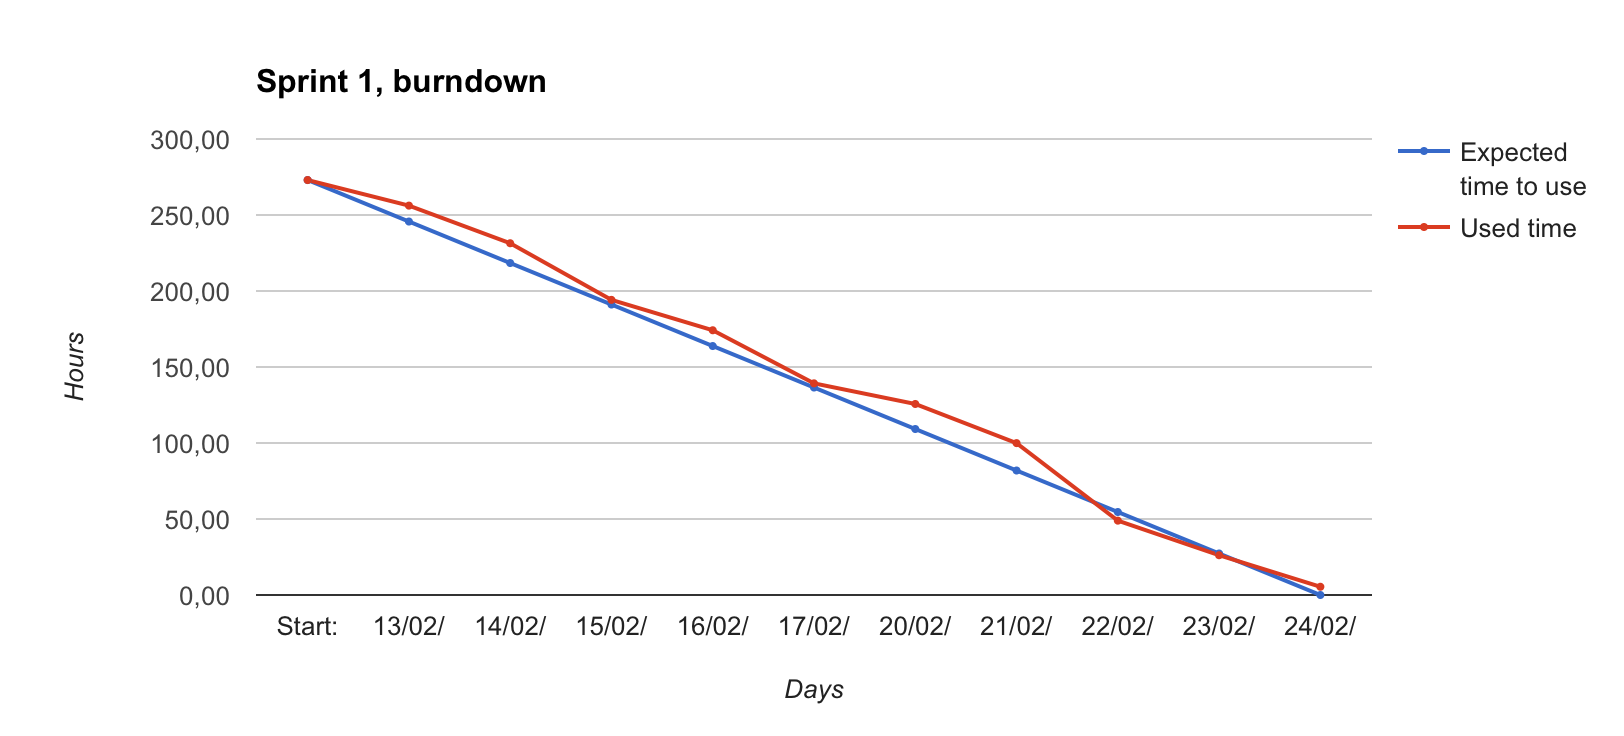
\includegraphics[width=\textwidth]{fig/sprint1}
    \caption{Sprint Burndown}
    \label{Hours_Worked_Burndown}
\end{figure}

\begin{figure}[H]
    \centering
    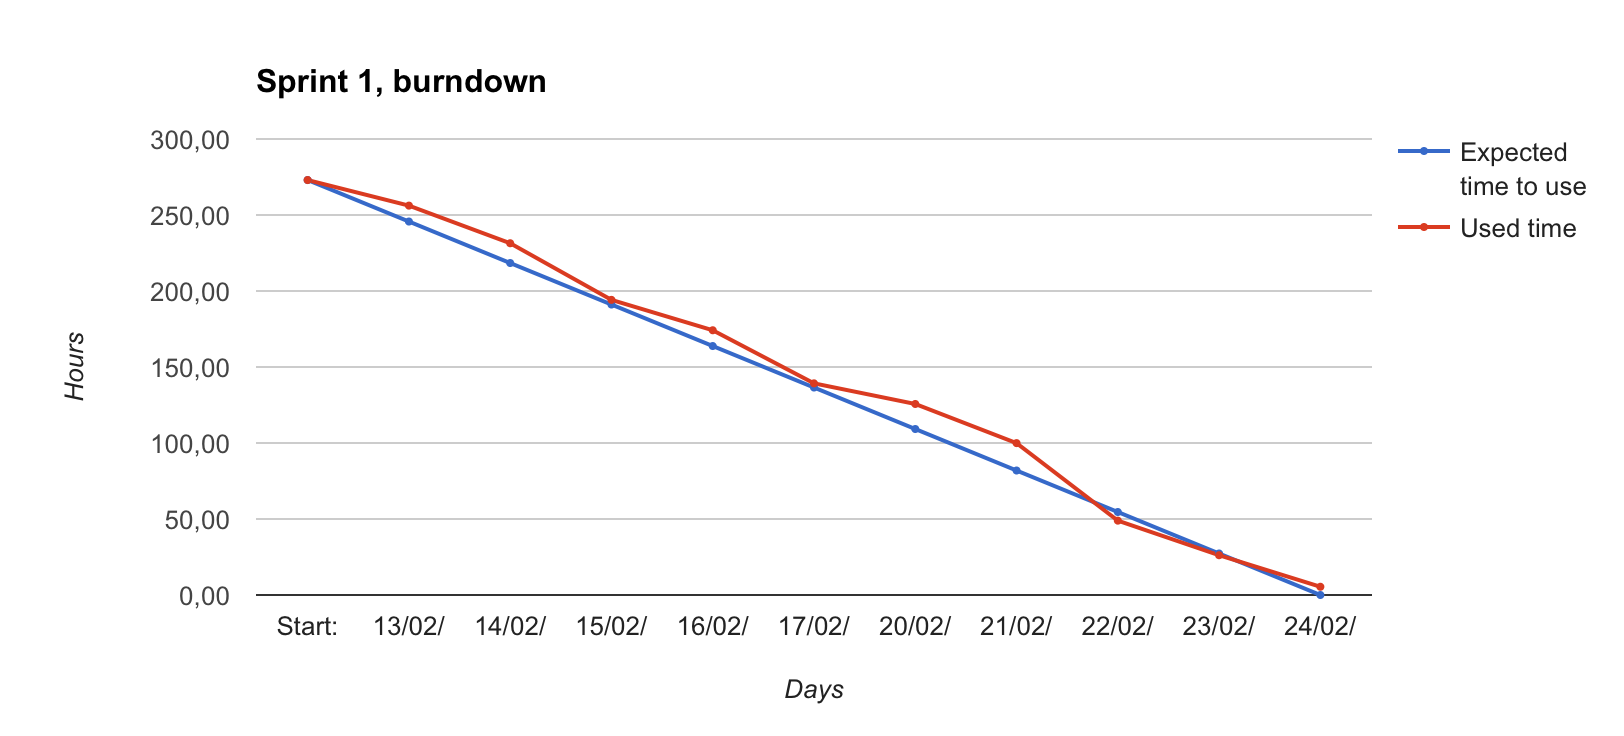
\includegraphics[width=\textwidth]{fig/sprint1}
    \caption{Distributed Time}
    \label{Distributed_Time}
\end{figure}

\section{Conclusion}
In the beginning of the project the had a workshop (see section \ref{WorkshopUserAndProviders}) with the users of the application. The workshop was used to gather as much information as possible, to actually understand what users wanted the application to do. The group organized all of the information so it was possible to make use of it. During the project the group used the customer actively to get feedback on how he thought the application should be. Together with the customer, group developed an application they thought would be suited for the users. 

In the end of sprint 4 (see section \ref{sprint4}) the group had a meeting (see section \ref{focusGrouoProviders}) with providers to see what they thought about the application. The providers was very happy with the result, and hoped that the development of the application would continue after the project was finished. In the beginning of sprint 4 (see section \ref{sprint5}) the group had a new workshop with the users (see section \ref{focusGroup}). This workshop turned out great. The users were very happy with the application and wanted the group to continue working on it. 

The group are very satisfied with the project. They have appreciated working with both a customer and different users. Throughout the entire project, the group has tried to satisfy both users and the customer, which it seems they have done. A final conclusion are that the group is pleased with the product they have developed, and it seems like both the users and the customer are satisfied with the product. 



\cleardoublepage